\documentclass[10pt,landscape]{article}
\usepackage{multicol}
\usepackage{calc}
\usepackage{ifthen}
\usepackage[landscape]{geometry}
\usepackage{hyperref}
\usepackage[]{algorithm2e}
\usepackage{graphicx}
\usepackage{xcolor}
\usepackage{listings}

% To make this come out properly in landscape mode, do one of the following
% 1.
%  pdflatex latexsheet.tex
%
% 2.
%  latex latexsheet.tex
%  dvips -P pdf  -t landscape latexsheet.dvi
%  ps2pdf latexsheet.ps


% If you're reading this, be prepared for confusion.  Making this was
% a learning experience for me, and it shows.  Much of the placement
% was hacked in; if you make it better, let me know...


% 2008-04
% Changed page margin code to use the geometry package. Also added code for
% conditional page margins, depending on paper size. Thanks to Uwe Ziegenhagen
% for the suggestions.

% 2006-08
% Made changes based on suggestions from Gene Cooperman. <gene at ccs.neu.edu>


% To Do:
% \listoffigures \listoftables
% \setcounter{secnumdepth}{0}



% This sets page margins to .5 inch if using letter paper, and to 1cm
% if using A4 paper. (This probably isn't strictly necessary.)
% If using another size paper, use default 1cm margins.
\ifthenelse{\lengthtest { \paperwidth = 11in}}
  { \geometry{top=.5in,left=.5in,right=.5in,bottom=.5in} }
  {\ifthenelse{ \lengthtest{ \paperwidth = 297mm}}
    {\geometry{top=1cm,left=1cm,right=1cm,bottom=1cm} }
    {\geometry{top=1cm,left=1cm,right=1cm,bottom=1cm} }
  }

% Turn off header and footer
\pagestyle{empty}
 
\lstset{language=Java}

% Redefine section commands to use less space
\makeatletter
\renewcommand{\section}{\@startsection{section}{1}{0mm}%
                                {-1ex plus -.5ex minus -.2ex}%
                                {0.5ex plus .2ex}%x
                                {\normalfont\large\bfseries}}
\renewcommand{\subsection}{\@startsection{subsection}{2}{0mm}%
                                {-1explus -.5ex minus -.2ex}%
                                {0.5ex plus .2ex}%
                                {\normalfont\normalsize\bfseries}}
\renewcommand{\subsubsection}{\@startsection{subsubsection}{3}{0mm}%
                                {-1ex plus -.5ex minus -.2ex}%
                                {1ex plus .2ex}%
                                {\normalfont\small\bfseries}}
\makeatother

\newcommand{\cfbox}[2]{%
    \colorlet{currentcolor}{.}%
    {\color{#1}%
    \framebox[1.1\width]{\color{currentcolor}#2}}%
}

% Define BibTeX command
\def\BibTeX{{\rm B\kern-.05em{\sc i\kern-.025em b}\kern-.08em
    T\kern-.1667em\lower.7ex\hbox{E}\kern-.125emX}}

% Don't print section numbers
\setcounter{secnumdepth}{0}


\setlength{\parindent}{0pt}
\setlength{\parskip}{0pt plus 0.5ex}


% -----------------------------------------------------------------------

\begin{document}

\raggedright
\footnotesize
\begin{multicols}{3}


% multicol parameters
% These lengths are set only within the two main columns
%\setlength{\columnseprule}{0.25pt}
\setlength{\premulticols}{1pt}
\setlength{\postmulticols}{1pt}
\setlength{\multicolsep}{1pt}
\setlength{\columnsep}{2pt}

\begin{center}
     \Large{\textbf{Big Discrete Cheat Sheet}} \\
\end{center}

\section{4 Decidability}
\subsubsection{Other Info}
\begin{itemize}
	\item Every context-free language is decidable	
	\item $E_{TM}$ is undecidable because we can reduce $A_{TM}$ to $E_{TM}$
\end{itemize}

\begin{description}
  \item[Symmetric difference] $L(C)$ = $(L(A) \cap \overline{L(B)})\cup(\overline{L(A)} \cap L(B))$
\end{description}

\subsection{Countability}
\begin{itemize}
	\item A set A is \underline{\textbf{countable}} if either it is finite or it has the same size as N.
	\item The set of real numbers is uncountable.
	\item some languages are not Turing-recognizable because there are uncountably many languages yet only countably many turing machines.
	\item For any undecidable language, either it or its complement is not Turing-recognizable.
	\item A language \underline{\textbf{is decidable}} iff it is Turing-recognizable and co-Turing-recognizable.
\end{itemize}

\section{5 Reducibility}
A \textbf{\textit{reduction}} is a way of converting one problem to another problem in such a way that a solution to the second problem can be used to solve the first problem.\\
In terms of computability theory, if A is reducible to B and B is decidable, A also is decidable. Equivalently, if A is undecidable and reducible to B, B is undecidable. \\

\subsubsection{Definitions}
\begin{description}
  \item[Definition 5.5] Let M be a Turing machine and w an input string. An \textbf{\textit{accepting computation history}} for M on w is a sequence of configurations, $C_{1},C_{2},...,C_{l}$ where $C_{1}$ is the start configuration of M, and each $C_{i}$ legally follows from $C_{i-1}$ according to the rules of M. A \textbf{\textit{rejecting computation history}} for M on w is defined similarly, except that $C_{l}$ is a rejecting configuration.
  \item[Definition 5.6] A \textbf{\textit{linear bounded automaton}} is a restricted type of Turing machine wherin the tape head isn't permitted to move off the portion of the tape containing the input. If the machine tries to move its head off either end of the input, the head stays where it is--in the same way that the head will not move off the left-hand end of an ordinary Turing machine's tape.
  \item[Definition 5.20] Language A is \textbf{\textit{mapping reducible}} to language B, written A $\leq_{m}$ B, if ther is a computeable function $f:\ \Sigma^{*} \rightarrow \Sigma^{*}$, where for every w, $w \in A \Longleftrightarrow f(w) \in B$ The function $f$ is called the reduction from A to B.
\end{description}

\subsubsection{Theorems}
\begin{description}
  \item[5.22] If A $\leq_{m}$ B and B is decidable, then A is decidable.
  \item[5.28] If A $\leq_{m}$ B and B is Turing-recognizable, then A is Turing-recognizable.
  \item[5.29] If A $\leq_{m}$ B and A is not Turing-recognizable, then B is not Turing-recognizable.
  \item[5.30] If $EQ_{TM}$ is neither Turing-recognizable nor co-Turing-recognizable. 
\end{description}

\subsubsection{Corollary}
\begin{description}
  \item[5.23] If A $\leq_{m}$ B and A is undecidable, then B is undecidable.
  \item[5.29] If A $\leq_{m}$ B and A is not Turing-recognizable, then B is not Turing-recognizable.
\end{description}

\subsection{References}
\subsubsection{Defenitions}
\begin{itemize}
	\item $A_{DFA} = \{\langle B,\omega\rangle | B\  is\ a\ DFA\ that\ accepts\ input\ string\ \omega\}$
	\item $A_{NFA} = \{\langle B,\omega\rangle | B\ is\ an\ NDA\ that\ accepts\ input\ string\ \omega\}$
	\item $A_{REX} = \{\langle R,\omega\rangle | R\ is\ a\ regex\ that\ generates\ string\ \omega\}$
	\item $E_{DFA} = \{\langle A\rangle | A\ is\ a\ DFA\ and\ L(A)\ = \emptyset\}$
	\item $EQ_{DFA} = \{\langle A,B\rangle | A\ and\ B\ are\ DFAs\ and\ L(A) = L(B)\}$
	\item $A_{CFG} = \{\langle G,\omega\rangle | G\ is\ a\ CFG\ that\ generates\ string\ \omega\}$
	\item $E_{CFG} = \{\langle G\rangle | G\ is\ a\ CFG\ and\ L(G) = \emptyset\}$
	\item $EQ_{CFG} = \{\langle G,H\rangle | G\ and\ H\ are\ CFGs\ and\ L(G) = L(H)\}$
	\item $A_{TM} = \{\langle M,\omega\rangle | M\ is\ a\ TM\ and\ M\ accepts\ \omega\}$
  \item $HALT_{TM} = \{\langle M,\omega\rangle | M\ is\ a\ TM\ and\ M\ halts\ on\ input\ \omega\}$
	\item $E_{TM} = \{\langle M\rangle | M\ is\ a\ TM\ and\ L(M) = \emptyset\}$
	\item $REGULAR_{TM} = \{\langle M\rangle | M\ is\ a\ TM\ and\ L(M)\ is\ a\ reg\ lang\}$
	\item $EQ_{TM} = \{\langle M_{1},M_{2}\rangle | M_{1}\ and\ M_{2}\ are\ TMs\ and\ L(M_{1}) = L(M_{2})\}$
	\item $A_{LBA} = \{\langle M,\omega\rangle | M\ is\ an\ LBA\ that\ accepts\ string\ \omega\}$
\end{itemize}

\subsubsection{Info Table}
\begin{tabular}{| l | c |}
    \hline                       
      $A_{DFA}$   & decidable \\ \hline
      $A_{NFA}$   & decidable \\ \hline
      $A_{REX}$   & decidable \\ \hline
      $E_{DFA}$   & decidable \\ \hline
      $EQ_{DFA}$  & decidable \\ \hline
      $A_{CFG}$   & decidable \\ \hline
      $E_{CFG}$   & decidable \\ \hline
      $EQ_{CFG}$  & undecidable \\ \hline
      $A_{TM}$    & undecidable \\ \hline
      $A_{TM}$    & Turing-recognizable \\ \hline
      $\overline{A_{TM}}$ & not Turing-recognizable \\ \hline
      $HALT_{TM}$ & undecidable \\ \hline
      $E_{TM}$ & undecidable \\ \hline
      $REGULAR_{TM}$ & undecidable \\ \hline
      $EQ_{TM}$ & undecidable \\ \hline
      $A_{LBA}$ & decidable \\ \hline
      $E_{LBA}$ & undecidable \\ \hline
      $ALL_{CFG}$ & undecidable \\ \hline
\end{tabular}

\rule{0.3\linewidth}{0.25pt}
\scriptsize

\section{Tite Solutions}
\subsection{3 Decidability}

\subsubsection{question a}

$\mathrm{L} = \{ \langle{ M_1, M_2 \rangle} | L(M_1) \cup L(M_2) = \emptyset \}$

Prove that L is undecidable by reducing $\mathrm{HALT}_TM$ to L.
$\mathrm{HALT}_TM \leq_M L$

Assume TM S decides L we will create a decider for $\mathrm{HALT}_{TM}$ H.

\begin{algorithm}[H]
 $H \langle{ M, w \rangle}$ \{

 create a TM $M'$ that does not accept w.

 boolean f = S$\langle{ M, M' \rangle}$
 
 return f

 \}
\end{algorithm}

Because we 

\subsubsection{question b}
$\mathrm{L} = \{ \langle{ M, S \rangle} | $ M is a standard TM and S is a finite set of strings of {0, 1} such that there exists some string t $\in$ S*, such that M accepts t  \}

Prove that L is undecidable.

Assume the contrary that L is decidable. Let TM M' decide membership in L. We will design a TM R to decide $A_{TM}$ using M'.

\begin{algorithm}[H]
 $R \langle{ M, w \rangle}$ \{

 create a TM $M_1$ such that if its input isn't w it rejects, If its input is w, it runs the steps of M.

 Thus, 

 L($M_1$) = $\emptyset$ if m doesn't accept w and

 L($M_1$) = \{w\} if m does accept w 

 \}
\end{algorithm}

If R accepts, then M' accepted. If M' accepts then a string of the form w* $\in$ L($M_1$). But L($M_1$) = \{w\} or L($M_1$) = $\emptyset$. It follows that if a string of the form w* $\in$ L($M_1$), then w $\in$ L($M_1$), which means M accepts w, as desired. Finally, when M' rejects we know w $\in$ L($M_1$) so M doesn't accept w in that case. This proves the correctness of R.

Since $A_{TM}$ is undecidable though, we can conclude that no decider for L exists. Hence, L is undecidable as desired. 



\subsubsection{c question}
$\mathrm{L} = \{ \langle{ D, M \rangle} | $ D is a DFA and M is a Turing Machine such that L(M) = L(D) \}

\section{Known Reduction}
\subsection{3-SAT to VERTEX COVER}
$\phi = (x_1 \vee x_1 \vee x_2) \wedge (\overline{x_1} \vee \overline{x_2} \vee \overline{x_2} ) \wedge (\overline{x_1} \vee x_2 \vee x_2)$
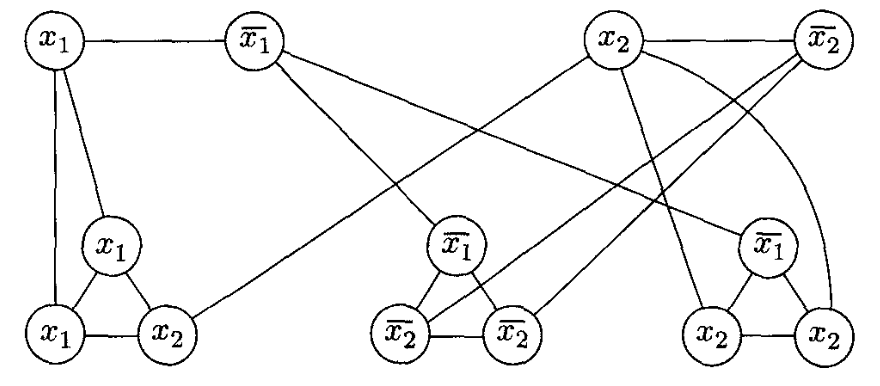
\includegraphics[width=0.8\linewidth]{satvc}\\
Circle the vertices that will minimally cover each edge

\subsection{3-SAT to CLIQUE}
\begin{enumerate}
  \item Pick an instance of 3-SAT with k clause
  \item Make a vertex for each literal
  \item Connect each vertex to the literals in other clause that are not the negation
  \item any k-clique in this graph corresponds to a satisfying assignment
\end{enumerate}

$\phi = (x_1 \vee x_1 \vee x_2) \wedge (\overline{x_1} \vee \overline{x_2} \vee \overline{x_2} ) \wedge (\overline{x_1} \vee x_2 \vee x_2)$

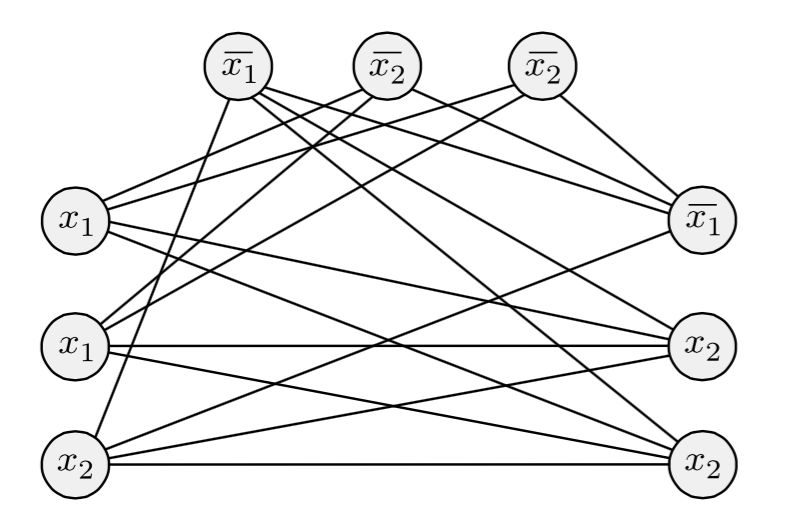
\includegraphics[width=0.8\linewidth]{satclique}

\subsection{Vertex-Cover to Subset-Sum}
Prove Subset-Sum is NP-Complete by mapping Vertex-Cover to Subset-Sum\\
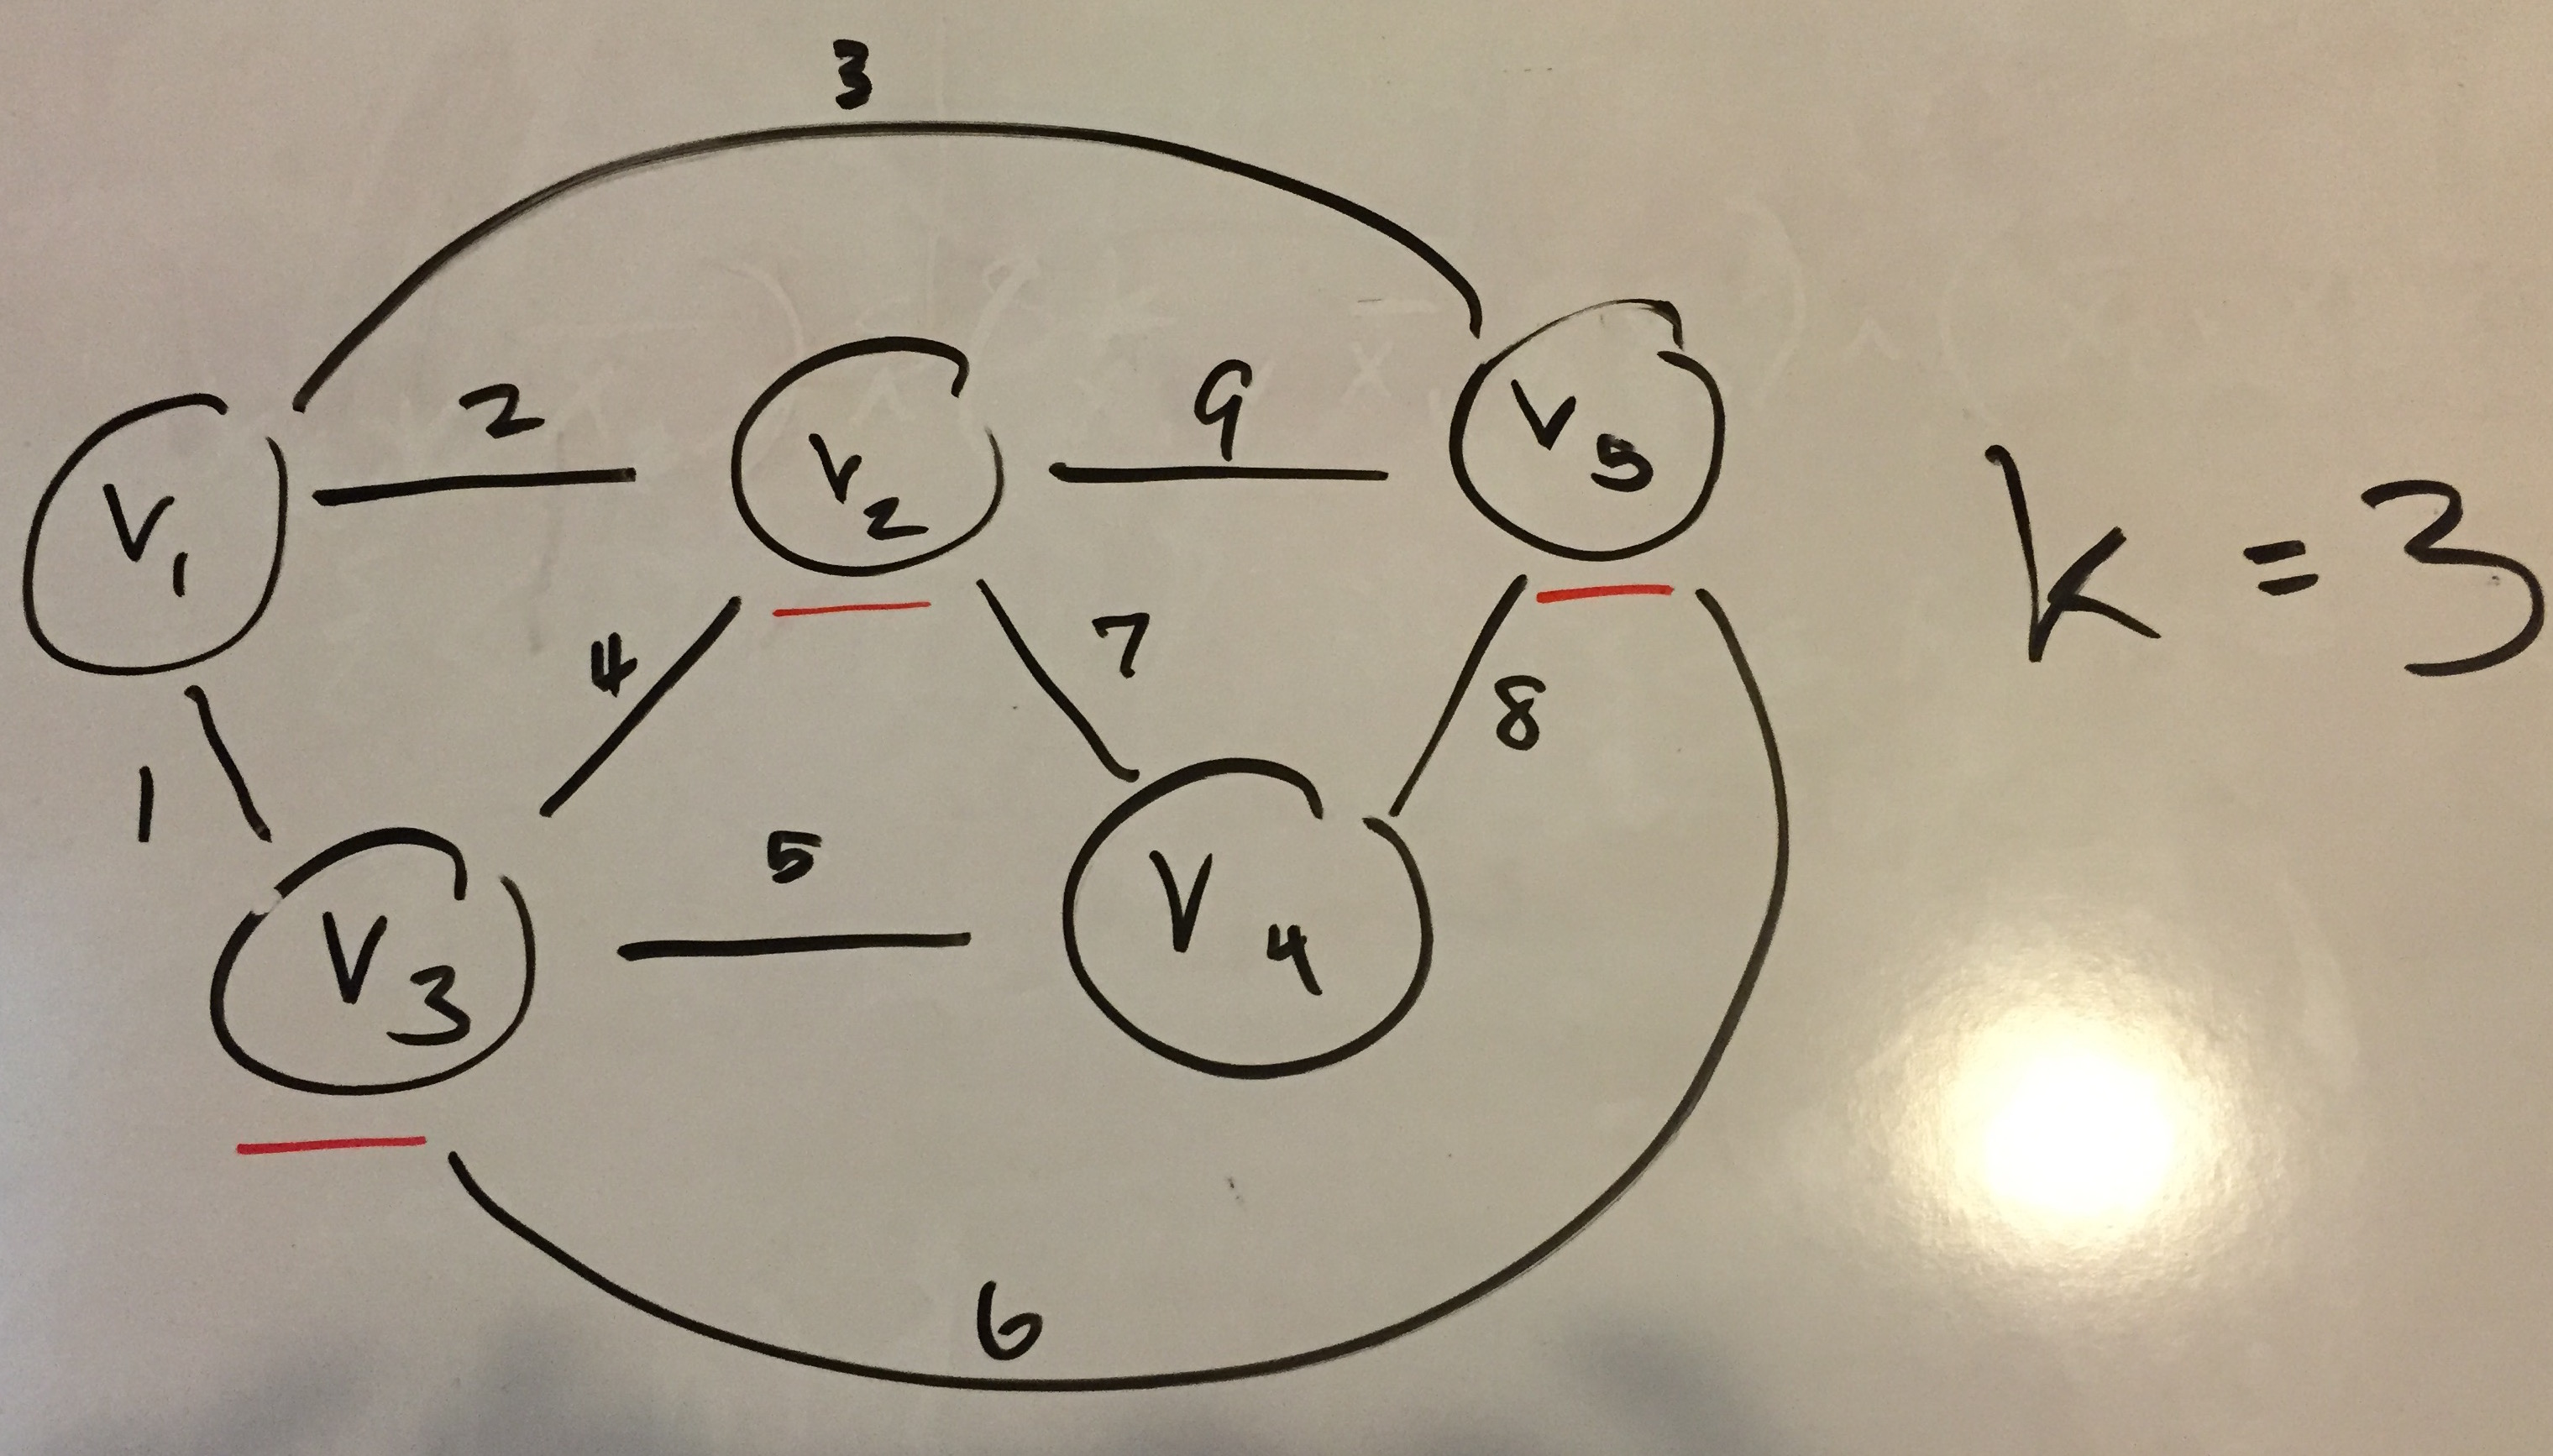
\includegraphics[width=0.8\linewidth]{vcss}
\begin{tabular}{l | l | l l l l l l l l l }
 & $x$ & $e_{1}$ & $e_{2}$ & $e_{3}$ & $e_{4}$ & $e_{5}$ & $e_{6}$ & $e_{7}$ & $e_{8}$ & $e_{9}$ \\ \hline
\hfill$v_{1}$ & 1 & 1 & 1 & 1 & 0 & 0 & 0 & 0 & 0 & 0 \\ \cline{2-11}
\hfill$v_{2}$ & \multicolumn{1}{|c|}{\cfbox{black}{1} \par} & 0 & \cfbox{black}{1} \par & 0 & \cfbox{black}{1} \par & 0 & 0 & \cfbox{black}{1} \par & 0 &\multicolumn{1}{c|}{\cfbox{black}{1} \par} \\ \cline{2-11}
\hfill$v_{3}$ & \multicolumn{1}{|c|}{\cfbox{black}{1} \par} & \cfbox{black}{1} \par & 0 & 0 & \cfbox{black}{1} \par & \cfbox{black}{1} \par & \cfbox{black}{1} \par & 0 & 0 & \multicolumn{1}{c|}{0} \\ \cline{2-11}
\hfill$v_{4}$ & 1 & 0 & 0 & 0 & 0 & 1 & 0 & 1 & 1 & 0 \\ \cline{2-11}
\hfill$v_{5}$ & \multicolumn{1}{|c|}{\cfbox{black}{1} \par} & 0 & 0 & \cfbox{black}{1} \par & 0 & 0 & \cfbox{black}{1} \par & 0 & \cfbox{black}{1} \par & \multicolumn{1}{c|}{\cfbox{black}{1} \par} \\ \cline{2-11}
\hfill$e_{1}$ & 0 & \cfbox{black}{1} \par & 0 & 0 & 0 & 0 & 0 & 0 & 0 & 0 \\ 
\hfill$e_{2}$ & 0 & 0 & \cfbox{black}{1} \par & 0 & 0 & 0 & 0 & 0 & 0 & 0 \\ 
\hfill$e_{3}$ & 0 & 0 & 0 & \cfbox{black}{1} \par & 0 & 0 & 0 & 0 & 0 & 0 \\ 
\hfill$e_{4}$ & 0 & 0 & 0 & 0 & 1 & 0 & 0 & 0 & 0 & 0 \\ 
\hfill$e_{5}$ & 0 & 0 & 0 & 0 & 0 & \cfbox{black}{1} \par & 0 & 0 & 0 & 0 \\ 
\hfill$e_{6}$ & 0 & 0 & 0 & 0 & 0 & 0 & 1 & 0 & 0 & 0 \\ 
\hfill$e_{7}$ & 0 & 0 & 0 & 0 & 0 & 0 & 0 & \cfbox{black}{1} \par & 0 & 0 \\ 
\hfill$e_{8}$ & 0 & 0 & 0 & 0 & 0 & 0 & 0 & 0 & \cfbox{black}{1} \par & 0 \\ 
\hfill$e_{9}$ & 0 & 0 & 0 & 0 & 0 & 0 & 0 & 0 & 0 & 1 \\ \hline
Target & 3 & 2 & 2 & 2 & 2 & 2 & 2 & 2 & 2 & 2 \\
\end{tabular} \\ \vspace{3pt} 

\subsection{3-SAT to SUBSET-SUM: Prove SS-SUM is NP-Complete}
$$
\left(x_{1} \vee x_{2} \vee \overline{x_{3}}\right)\wedge\left(\overline{x_{1}}\vee x_{2}\vee \overline{x_{3}}\right)\wedge\left(x_{1}\vee \overline{x_{2}}\vee x_{3}\right)\wedge\left(\overline{x_{1}}\vee \overline{x_{2}}\vee \overline{x_{3}}\right)
$$
$$3-SAT \leq_{p} SUBSET-SUM$$
We can reduce 3-SAT to SUBSET-SUM by representing the variables and clauses in a table. We encode the selection of truth values into a subset sum problem as follows: \\ 
\begin{tabular}{l | l l l | l l l r }
& \multicolumn{3}{ c| }{Vars} & \multicolumn{4}{ |c }{Clauses} \\
 & 1 & 2 & 3 & 1 & 2 & 3 & 4 \\ \hline
\hfill $x_{1}$ & 1 & 0 & 0 & \framebox[1.1\width]{1} \par & 0 & \framebox[1.1\width]{1} \par & 0 \\
\hfill $\overline{x_{1}}$ & 1 & 0 & 0 & 0 & 1 & 0 & 1 \\
\hfill $x_{2}$ & 0 & 1 & 0 & \cfbox{black}{1} & \framebox[1.1\width]{1} \par & 0 & 0 \\
\hfill $\overline{x_{2}}$ & 0 & 1 & 0 & 0 & 0 & \cfbox{green}{1} \par & \cfbox{green}{1} \par \\
\hfill $x_{3}$ & 0 & 0 & 1 & 0 & 0 & 1 & 0 \\
\hfill $\overline{x_{3}}$ & 0 & 0 & 1 & \framebox[1.1\width]{1} \par & \framebox[1.1\width]{1} \par & 0 & \framebox[1.1\width]{1} \par \\ \hline
\hfill $S_{1a}$ & 0 & 0 & 0 & 1 & 0 & 0 & 0 \\
\hfill $S_{1b}$ & 0 & 0 & 0 & 1 & 0 & 0 & 0 \\
\hfill $S_{2a}$ & 0 & 0 & 0 & 0 & \framebox[1.1\width]{1} \par & 0 & 0 \\
\hfill $S_{2b}$ & 0 & 0 & 0 & 0 & 1 & 0 & 0 \\
\hfill $S_{3a}$ & 0 & 0 & 0 & 0 & 0 & \framebox[1.1\width]{1} \par & 0 \\
\hfill $S_{3b}$ & 0 & 0 & 0 & 0 & 0 & \framebox[1.1\width]{1} \par & 0 \\
\hfill $S_{4a}$ & 0 & 0 & 0 & 0 & 0 & 0 & \framebox[1.1\width]{1} \par \\
\hfill $S_{4b}$ & 0 & 0 & 0 & 0 & 0 & 0 & \framebox[1.1\width]{1} \par \\ \hline
Target & 1 & 1 & 1 & 3 & 3 & 3 & 3 \\
\end{tabular} \\ \vspace{3pt} 
$x_{1}$ = True \\
$x_{2}$ = True or False (denoted by a green box) \\
$x_{3}$ = False \\
$C_{1}$ = 3 = 3 \\
$C_{2}$ = 2 + 1 = 3\\
$C_{3}$ = 1 + 2 = 3\\
$C_{4}$ = 1 + 2 = 3\\
By computing the subset sum of each of the columns where Target is the bottom row we can solve Subset-Sum if we can solve 3-SAT\\

\subsection{SUBSET-SUM to SUBSET-SUM-K}
$$SUBSET\mbox{-}SUM \leq_{p} SUBSET\mbox{-}SUM\mbox{-}k$$\\
\hspace{5pt}$SUBSET$-$SUM\langle S,T \rangle\{$\\
\hspace{10pt}$SUBSET$-$SUB \in NP$ because we can verify a certificate in\\ \hspace{92pt}linear time. Given an answer you can\\ \hspace{92pt}verify it adds up to T and all of the\\ \hspace{92pt}elements of our subset are in our\\ \hspace{92pt}original set\\
\hspace{10pt}$S=\{x_{1}, x_{2}, \ldots, x_{n}\}$\\
\hspace{10pt}$Y=\sum\limits_{i=0}^{n}x_{i}$\\
\hspace{10pt}$S' = \{Y,\ldots,Y_{n}, Y-x_{1}, Y-x_{2}, \ldots, Y-x_{n}\}$ where $|S'| = 2n$\\
\hspace{10pt}$T' = nY-T$\\
\hspace{10pt}$k=n$\\
$\}$\\
$S'$ is the set of n Y's and a Y minus each x value \\
$T'$ is n numbers of Y's and you subtract your T value which is the x's you chose\\
our k is now equal to n in our subset-sum-k\\
$$SUBSET\mbox{-}SUM\mbox{-}k \leq_{p} SUBSET\mbox{-}SUM$$\\
\begin{enumerate}
\item $mY+(n-m)Y-(x for x \in soln) = nY-T$\\
\item $(x\ for\ x \in soln) = T$\\
\end{enumerate}

\section{Greedy/DP Problems}
\subsection{Dinner Problem}
\begin{lstlisting}
Public Static void main(String[] args){
  memo = new long[n+1];
  Arrays.fill(memo, -1);
  memo[0] = 0;
  long ans = ans(n);
}
static long ans(int n){
  if(n <= 0) //base case 1
    return n == 0 ? 1 : 0;
  if(memo[n] != -1) //base case 2: check the memo
    return memo[n];
  long ans = 0;
  ans += ans(n-2) + ans(n-5) + ans(n-10);
  return memo[n] = ans; //save the answer
}
\end{lstlisting}
%Copyright \copyright\ 2015 Conner Brooks 
\vspace{5pt}
\href{http://github.com/connerbrooks/cheat-sheets}{http://github.com/connerbrooks/cheat-sheets}\\
Greetz to my bud \href{http://github.com/broglea}{brogle... He did the zweet table}.

\end{multicols}
\end{document}
